\documentclass[12pt]{report}
%PAQUETES BASICOS------------------------
\usepackage[utf8]{inputenc}
\usepackage[spanish]{babel}
\usepackage[left=2cm,right=2cm,top=2cm,bottom=2cm]{geometry}
%TEXTO DE PRUEBA------------------------
\parindent=0cm
\usepackage{amsmath}
\usepackage{amssymb,amsfonts,latexsym,cancel}
\usepackage{esvect}
\usepackage{txfonts}
\usepackage{array}
\usepackage{float}
\usepackage{fancyhdr}
\usepackage{graphicx}
\usepackage[colorlinks=true,linkcolor=blue,citecolor=black,urlcolor=blue]{hyperref}
\setcounter{MaxMatrixCols}{40}
\usepackage{multicol,multirow,booktabs}
\usepackage{subfigure}
\usepackage{titling}
\usepackage{titlesec}
\usepackage{anyfontsize}
\usepackage{listings}
%--------------------------------------------------
%Interlineado
\renewcommand{\baselinestretch}{1.5}
%--------------------------------------------------
%Estilo de pagina
\pagestyle{fancy}
\fancyhead{}%
\fancyhead[L]{Aplicación de ecuaciones diferenciales de Primer Orden}
\fancyhead[R]{
\includegraphics[scale=0.05]{ESCUDO UC.jpg}}
\fancyfoot{}
\fancyfoot[R]{\thepage}
\fancyfoot[L]{\footnotesize{Laura Natalia Ordoñez Chicangana}}
\renewcommand{\headrulewidth}{0.5pt}
\renewcommand{\footrulewidth}{0.5pt}
\setcounter{tocdepth}{3}

\newcommand{\limite}[2]{\mathop{\underset{n\to #1}{\mathrm{lim}}\ #2}}

\newcommand{\xan}[1]{\mathop{\textcolor{red}{\cancel{#1}}}}

\newcommand{\absg}[1]{\mathop{\bigl| #1 \bigr|}}
\newcommand{\absgg}[1]{\mathop{\biggl| #1 \biggr|}}
\newcommand{\absggg}[1]{\mathop{\Biggl| #1 \Biggr|}}

%--------------------------------------------------
%PARENTESIS
%--------------------------------------------------
\newcommand{\parg}[1]{\mathop{\big( #1 \big)}}
\newcommand{\pargg}[1]{\mathop{\bigg( #1 \bigg)}}
\newcommand{\parggg}[1]{\mathop{\Bigg( #1 \Bigg)}}
%--------------------------------------------------
%CORCHETES
%--------------------------------------------------
\newcommand{\corg}[1]{\mathop{\big[ #1 \big]}}
\newcommand{\corgg}[1]{\mathop{\bigg[ #1 \bigg]}}
\newcommand{\corggg}[1]{\mathop{\Bigg[ #1 \Bigg]}}
%--------------------------------------------------
%LLAVES
%--------------------------------------------------
\newcommand{\lag}[1]{\mathop{\big\{ #1 \big\}}}
\newcommand{\lagg}[1]{\mathop{\bigg\{ #1 \bigg\}}}
\newcommand{\laggg}[1]{\mathop{\Bigg\{ #1 \Bigg\}}}


\begin{document}

\begin{titlepage}
\centering
{\bfseries\LARGE Universidad del Cauca \par}
\vspace{0.1cm}
{\bfseries\LARGE Facultad de Ingeniería Civil \par}
\vspace{0.1cm}
{\bfseries\LARGE Programa: Ingeniería Civil \par}
\vspace{0.2cm}


\includegraphics[scale=0.3]{ESCUDO UC.jpg}

{\scshape\Huge Aplicación de Ecuaciones Diferenciales de Primer Orden \par}
\vspace{1cm}

{\bfseries\Large Presentado por: \par}
{\Large Laura Natalia Ordoñez Chicangana \par}
{\bfseries\Large Código: \par}
{\Large 100417011049 \par}
{\bfseries\Large Presentado a: \par}
{\Large Profesor Jhonatan Collazos Ramírez \par}

\vfill
{\Large Popayán, agosto de 2022 \par}
\end{titlepage}
\newpage

\title{Aplicación de Ecuaciones Diferenciales de Primer Orden}
\author{Laura Natalia Ordoñez Chicangana}
\date{Popayán, agosto de 2022}
\maketitle
\tableofcontents

\begin{abstract}
En este artículo se realizará el desarrollo teórico de una aplicación relacionada con epidemiología, en la cual se seguirán varías hipótesis para restringir el comportamiento con que una enfermedad se puede contagiar. Para dar sustento a este modelo teórico, se va a realizar la ejecución de un script en \href{https://www.mathworks.com/products/matlab.html}{MATLAB} que nos permitirá verificar la solución que obtendremos analíticamente con los métodos convencionales de solución para Ecuaciones diferenciales de primer orden.
\end{abstract}

\newpage

\section{Introducción}
Una ecuación diferencial ordinaria de primer orden es una ecuación diferencial ordinaria donde intervienen derivadas de primer orden respecto a una variable independiente. Es una relación en la que intervienen la variable dependiente, la función incógnita y su derivada de primer orden.

Las ecuaciones diferenciales tienen múltiples aplicaciones y son una gran herramienta matemática para describir situaciones o fenómenos reales, pero para que sean realmente útiles necesitamos saber resolverlas y que no todas tienen solución.

En nuestro artículo trataremos una enfermedad existente debido al surgimiento actual de la pandemia, surge un problema básico que pretende describir mediante el uso de una Ecuación Diferencial de Primer Orden, el comportamiento de una pequeña epidemia regida por ciertas restricciones hipóteticas que permitan establecer en el dominio del tiempo como sería el desempeño de esta situación en una localidad con cierto número de habitantes.

La ejecución de este pequeño ejercicio hipótetico es clave porque permite establecer un escenario y lo más importante, establecer una curva en el dominio del tiempo que permita establecer cuántos habitantes de la población están infectados, lo cual no tiene que ver con los objetivos del ejercicio, pero en la vida real constituye una manera útil de realizar pronósticos y ejecutar tomas de decisiones para eventualidades en materia de salud.


En cuanto a la ecuación diferencial que se pretende resolver se le conoce como Modelo de Crecimiento Logistico, este modelo entra en la categoría de ecuaciones diferenciales de primer orden, donde la tasa de cambio de los individuos es directamente proporcional a dos poblaciones que tienen caracteristicas distintas, es decir, en el caso de un modelo de epidemiología, la población sana junto a la población infectada por el agente contagioso. Este modelo ademas exige la presencia de una constante de proporcionalidad.

\newpage

\section{Modelo para epidemiología}
Antes de comenzar a proponer ecuaciones, debemos restringir un poco el comportamiento de este modelo con ciertas hipótesis que vamos a listar a continuación:
\begin{itemize}
\item La población es un número que se mantiene fijo, esto quiere decir que la suma de individuos infectados y sanos dara siempre como resultado la población bajo estudio la cual llamaremos $P$.
\item El caso que estudiamos, se trata de una enfermedad que es larga, la cual no se cura en el dominio de tiempo, esto quiere decir que estaremos estudiando un modelo en tiempo en el que las personas sólo se infectan, no consideramos en ningún momento que hayan individuos curándose.
\item Debido a la hipótesis anterior no se puede obviar el hecho de que estos individuos infectados, circulan libremente entre la población $P$, de manera que esta mezcla entre individuos sanos e infectados solo origina mas contagios.
\item Durante cada unidad de tiempo cada persona infectada tienen un número de $c$ contactos y cada contacto con una persona no infectada redunda en la transmisión de la enfermedad.
\end{itemize}

\newpage

\section{Modelo teórico}
Sea $f\parg{t}$ la función que gobierna a la población de individuos infectados para un instante de tiempo $t$, entonces la razón de cambio para las infecciones será proporcional a la población infectada como la población sana y el coeficiente de contactos que denotamos $c$. De este modo la ecuación que gobierna el problema es la siguiente:

\begin{equation}\label{ecuacion 1}
\frac{df}{dt}=\frac{c}{P} f\parg{P-f}
\end{equation}

La ecuación \ref{ecuacion 1} es una ecuación diferencial de primer orden que puede ser abordada por el método de variables separables como sigue:

$$\frac{df}{f\parg{P-f}}=\frac{c\ dt}{P}$$
$$\int\frac{df}{f\parg{P-f}}=\int\frac{c\ dt}{P}$$

Aplicamos el método de fracciones parciales y nos queda:
$$\frac{1}{f\parg{P-f}}=\frac{1}{f P}-\frac{1}{P\parg{f-P}}$$

Sustituyendo eso en el integrando nos queda:
$$\int\parggg{\frac{1}{f P}-\frac{1}{P\parg{f-P}}}df=\int\frac{c\ dt}{P}$$

Realizamos la operación de integración y nos queda:
$$\frac{1}{P} Ln\absgg{\frac{f}{f-P}}=\frac{ct}{P}+K$$
$$Ln\absgg{\frac{f}{f-P}}=ct+PK$$

Despejamos la función $f$ y respetando las propiedades del valor absoluto, nos queda:
$$\frac{f}{P-f}=e^{PK+ct}$$
$$f=Pe^{PK+ct}-fe^{PK+ct}$$
$$f\parg{1+e^{PK+ct}}=Pe^{PK+ct}$$

De esta forma la solución al problema es:
\begin{equation}\label{ecuacion 2}
f\parg{t}=\frac{Pe^{PK+ct}}{e^{PK+ct}+1}
\end{equation}

\newpage

Un aspecto importante que debemos destacar es que la constante $K$ viene de las condiciones iniciales del problema, en nuestro caso, tenemos que considerador que $f\parg{0}<P$, con esa condición es posible hallar el valor de $K$
\section{Ejemplo}
Supongamos la situación en que en una ciudad aislada de 300000 personas, solo opera un centro de salud. Durante el comienzo de la primera semana en que se observó el primer caso de una enfermedad contagiosa, se resgistraron 50 casos con un coeficiente de contactos de $0.85$.

Identificando los datos del problema, podemos ver que:
$$f\parg{0}=50$$

Esto en la ecuacion \ref{ecuacion 2} se traduce en:
$$\frac{1}{300000} Ln\absgg{\frac{50}{50-300000}}=K$$
$$K=-\frac{Ln\parg{5999}}{300000}$$

Por lo tanto la función que gobierna el número de personas infectadas es:
$$f\parg{t}=\frac{300000 e^{0.85t-Ln\parg{5999}}}{e^{0.85t-Ln\parg{5999}}+1}$$
$$f\parg{t}=\frac{300000 e^{0.85t}}{e^{0.85t}+5999}$$

Si quisieramos el valor de la población infectada al cabo de 12 semanas, sería:
$$f\parg{12}=\frac{300000 e^{0.85\cdot 12}}{e^{0.85\cdot 12}+5999}\approx 245000$$

\newpage

\section{Verificación en MATLAB}
En la lista de código subidos a la plataforma GITHUB se encuentra el archivo .m script de MATLAB.
La verificación en MATLAB se hará directamente en la aplicación, se adjunta el código que se va a ejecutar. 

Los comandos que se usaron para llevar a cabo nuestra verificación del problema son comandos sencillos. El primer comando "$syms$" lo usamos para declarar más de una variable simbólica, en nuestro caso y(t), $P$, $K$ y $C$.

Seguidamente se plantea la ecuación con el comando "$eqn$", utilizamos "$diff$" para encontrar la derivada de nuestra ecuación con más de una variable, lo comparamos con nuestra expresión usando el comando "$==$"

Con el comando $cond$ asignamos condiciones a nuestras variables, igualamos nuestras ecuaciones y con el comando $dsolve$ el programa MATLAB resuelve una ecuación diferencial ordinaria o un sistema de ecuaciones diferenciales.

Para hacer un gráfico usamos la función $plot$, tiene un compartamiento especial ya que depende del tipo de dato que se le asigne o se dé como argumento se generará diferente un tipo de gráfica, adicional a esto para una gráfica se puede poner el comando $grind on$ para ponerle una especie de rejilla o división para poder observar mejor los datos.

Finalmente con $round$ redondea cada elemento al más próximo.

Código ejecutado en MATLAB:



\begin{lstlisting}
syms y(t) P K c
eqn = diff(y,t) == (c/P)*y*(P-y);
cond = y(0) == K;
ySol(t) = dsolve(eqn,cond)
K=50;
P=300000;
c=0.85;
fplot(subs(ySol(t)),[0,25]);
grid on
round(subs(ySol(t)))
round(subs(ySol(12)))
\end{lstlisting}


\newpage

La salida del código es la siguiente en el prompt:
\begin{figure}[H]
\centering
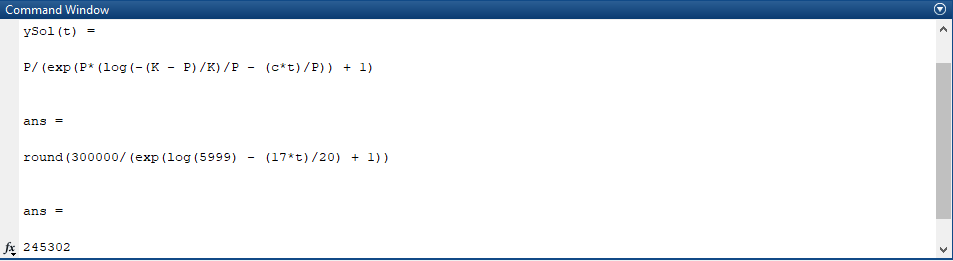
\includegraphics[scale=0.9]{IMAGEN SALIDA.png}
\caption{Ejecucion del Script.}\label{IMAGEN SALIDA}
\end{figure}

\begin{figure}[H]
\centering
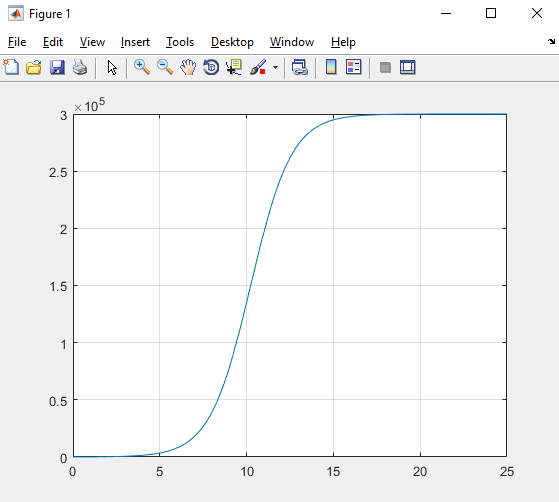
\includegraphics[scale=0.9]{IMAGEN GRAFICA SOLUCION.png}
\caption{Gráfica de la solución de la ecuación diferencial.}\label{IMAGEN GRAFICA SOLUCION}
\end{figure}
\newpage

\begin{thebibliography}{10}
\bibitem{Interes} \href{https://es.khanacademy.org/math/ap-calculus-bc/bc-differential-equations-new/bc-7-9/v/logistic-differential-equation-intuition#:~:text=La%20ecuaci%C3%B3n%20diferencial%20log%C3%ADstica%20dN,cuando%20alcanza%20el%20tama%C3%B1o%20K.}{El modelo de crecimiento logístico}
\bibitem{Epidemiología} \href{https://sites.google.com/site/rgnecuacionesdiferenciales/home/parcial-3/modelo-logistico}{Modelo logistico}
\bibitem{Funcion} \href{https://es.wikipedia.org/wiki/Funci%C3%B3n_log%C3%ADstica}{Funcion logistica}
\bibitem{MATLAB1} \href{https://www.mathworks.com/matlabcentral/answers/351952-plotting-a-result-from-dsolve}{Plotting a result from dsolve}
\bibitem{Denis} D. Zill; {\it Ecuaciones Diferenciales con  Aplicaciones de Modelado 9na Edición - Pagina 94}. CENGAGE. 2009
\end{thebibliography}

\end{document}